\documentclass[12pt]{article}

\usepackage{orcidlink}
\usepackage{amssymb}
\usepackage{physics}
%\usepackage{cite}
\usepackage{hyperref} % for hyperlinks in references
\usepackage[nameinlink]{cleveref}

\textwidth 150mm
\textheight 240mm
\voffset = -20mm

%Title of paper
\title{Pair distribution function for a cell model with Curie-Weiss interaction}

\author{R.V.~Romanik, M.P.~Kozlovskii, O.A.~Dobush
	\\ \small Institute for Condensed Matter Physics, NAS of Ukraine 
	\\ \small 1~Svientsitskii Street, 79011, Lviv, Ukraine 
	\\ \small romanik@icmp.lviv.ua}
%\author{R.V.~Romanik \\ Institute for Condensed Matter Physics, NAS of Ukraine}

\begin{document}
	
	\maketitle
	
	%\begin{multicols}{2}
	
	\abstract{In this paper we present results for the pair distribution function for a cell model with Curie-Weiss interaction
		\\
		
		\textbf{Keywords: } Pair distribution function, $n-$particle density, Curie-Weiss interaction, cell model.
	}
	
	\section{Introduction}
	
	\section{\label{sec:model} Model}
The cell model introduced and described in~\cite{KKD2018book,KKD2020} is considered. This model possesses an exact solution in the case of Curie-Weiss interaction. The exact asymptotic expressions for the grand partition function were obtained in~\cite{KKD2020}. In this paper we will study structure properties of the model, in particular $1$-body and $2$-body densities, and the pair distribution function.

Let us briefly introduce notation to be used in this paper, and then summarize the known results for the model.

We work within the formalism of the grand canonical ensemble. We consider a system of point particles contained in volume $V$. The volume $V$ is divided into a number of $N_v$ congruent cubic cells $\Delta_l$ of volume $v=c^3$, such that the volume $V$ is the union of all $\Delta_l$
\begin{equation*}
	V = \bigcup_{l=1}^{N_v}\Delta_l,
\end{equation*}
and for each pair of $\Delta_l$ and $\Delta_m$
\begin{equation*}
	\Delta_l \cap \Delta_m = \emptyset, \text{ if } l \neq m.
\end{equation*}

The interaction energy between particles in configuration $\gamma = \{x_1, ..., x_N\}$, where $x_i$ is the space coordinate of the $i$-th particle and $N$ is the number of particles in the configuration $\gamma$, is defined as follows
\begin{equation*}
	W_{N_v}(\gamma) = \frac{1}{2} \sum_{x,y \in \gamma} \Phi_{N_v} (x,y)
\end{equation*}
where $\Phi_{N_v}$ is given by the Curie-Weiss interaction
\begin{equation}
	\label{def:curie-weiss-pot}
	\Phi_{N_v}(x, y) = -\frac{J_1}{N_v} + J_2\sum_{l=1}^{N_v} I_{\Delta_l}(x) I_{\Delta_l}(y),
\end{equation}
and $I_{\Delta_l}(x)$ is the indicator of $\Delta_l$
\begin{equation*}
	I_{\Delta_l} (x) = \left\{
	\begin{array}{ll}
		1, \quad x \in \Delta_l,
		\\
		0, \quad x \notin \Delta_l.
	\end{array}
	\right.
\end{equation*}
The first term in $\Phi_{N_v}$ describes the pairwise attraction between all particles and is characterized by $J_1 > 0$. The second term in $\Phi_{N_v}$ describes the repulsion between two particles contained within the same cell $\Delta_l$ and is characterized by $J_2 > 0.$ For stability of interaction the following condition must hold
\begin{equation*}
	J_2 > J_1.
\end{equation*}
Let us introduce notation
$$a = J_2/J_1.$$
In this work we fix $a=1.2$.

The grand partition function is defined as follows
\begin{equation*}
	\Xi = \sum_{N=0}^{\infty}\frac{z^N}{N!} \int_{V} \dotsc \int_{V} \exp(-\beta W_{N_v}(\gamma)) {\rm d} x_1 \dotsc {\rm d} x_N
\end{equation*}
where $z$ is the activity
\begin{equation*}
	z = \frac{\exp(\beta \mu)}{\Lambda^3},
\end{equation*}
$\beta = k_{\rm B} T$ the inverse temperature, $k_{\rm B}$ Boltzmann constant, $T$ the temperature, $\mu$ the chemical potential, $\Lambda = (2\pi\beta\hbar^2/m)^{1/2}$ the de Broglie thermal wavelength, $\hbar$ the Planck constant, $m$ the mass of a particle. In the grand partition function the integration goes over all configurations with $N$ particles and then the summation goes over all positive integer values of $N$.

Natural units for energy and length in our model are $J_1$ and $c$, respectively. It is standard practice to present thermodynamic results in terms of dimensionless quantities, normalized by the natural units. The usefulness of such quantities is that their numerical values are usually of the order of unity. Thus we introduce the following reduced quantities: 

%the reduced temperature $T^* = k_{\rm B} T / J_1$, the reduced inverse temperature $p = \beta J_1$, reduced chemical potential $\mu^* = \mu / J_1$, and the reduced pressure $P^* = Pv/J_1$.
\begin{eqnarray*}
	T^* = \frac{k_{\rm B} T}{J_1} & \quad & \text{ -- the reduced temperature;} 
	\\
	p = \beta J_1 = \frac{1}{T^*} & \quad & \text{ -- the reduced inverse temperature;}
	\\
	\mu^* = \frac{\mu}{J_1} & \quad & \text{ -- the reduced chemical potential;}
	\\ 
	P^* = \frac{Pv}{J_1} & & \text{ -- the reduced pressure;}
\end{eqnarray*}

In works~\cite{KKD2018book,KKD2020} the following expression was obtained for the grand partition function
\begin{equation}
	\Xi \simeq c_{N_v} \exp[N_v E(\bar{y}, p, \mu)]
\end{equation}
which is asymptotically exact for the limit of $N_v \to \infty$. Here $\bar{y}$ is a function of both $p$ and $\mu$ and is found from the condition of maximum for quantity $E$, which is defined as follows
\begin{equation*}
	E(y, p, \mu) = -\frac{y^2}{2p} + \ln K_0(y,p,\mu),
\end{equation*}
where $K_0(y,p,\mu)$ is the $0$-th member of the following family of special functions
\begin{equation*}
	K_m(y,p,\mu) = \sum_{n=0}^{\infty} \frac{n^m v^n}{n!} \exp[(y+\mu)n - \frac{a p}{2}n^2].
\end{equation*}
For detailed investigation of the conditions necessary for the global maximum of $E$ and the derivation of relations for $\bar{y}$, we direct the interested readers to works~\cite{KKD2018book,KKD2020,MpkDob2022}. In this study we employ the methodology developed and the results derived in those works to investigate the pair distribution function. 

	
	\section{\label{sec:init-pair-distribution} Pair distribution function}
The $n$-particle distribution function is defined via $n$-particle densities as follows (for reference, see Section~2.6 in~\cite{hansen2013theory})
\begin{equation*}
	\label{def:g_n}
	g^{(n)}(x_1,\dotsc,x_n)=\frac{\rho^{(n)}(x_1,\dotsc,x_n)}{\prod_{i=1}^{n}\rho^{(1)}(x_i)}
\end{equation*}
where $n$-particle density defined in the grand canonical ensemble is
\begin{eqnarray*}
	\label{def:rho_n}
	\rho^{(n)}(x_1,\dotsc,x_n) = \frac{1}{\Xi}\sum_{N=n}^{\infty} \frac{z^N}{(N-n)!} \int\exp(-\beta W_{N_v}(\gamma)) {\rm d} x_{n+1} \dotsc {\rm d} x_N.
\end{eqnarray*}
In this work, our goal is to calculate the pair distribution function $g^{(2)}(x_1, x_2)$
\begin{equation*}
	g^{(2)}(x_1, x_2) = \frac{\rho^{(2)}(x_1, x_2)}{\rho^{(1)}(x_1) \rho^{(2)}(x_2)}.
\end{equation*}
Thus we first need to calculate the one- and two-particle densities.

Let us first calculate $\rho^{(1)}$. By definition
\begin{equation*}
	\rho^{(1)} (x_1) = \Xi^{-1} \sum_{N=1}^{\infty} \frac{z^N}{(N-n)!} \int \exp(-\beta W_{N_v}(x_1, \dotsc, x_N)) {\rm d} x_2 \dotsc {\rm d} x_N.
\end{equation*}
Applying the method described in~\cite{KKD2020}, we obtain the following result
\begin{equation*}
	\rho^{(1)} (x_1) = \frac{K_1(\bar{y}, p, \mu)}{v K_0(\bar{y},p,\mu)} = \frac{\bar{n}(p,\mu)}{v}
\end{equation*}
where $\bar{n}$ is the average value of the occupation number of a cell. Thus, for the considered cell model with Curie-Weiss interaction we obtained the result known for homogeneous systems: the single-particle density is equal to the average particle density. In the presented theory, the average values are calculated using the probability measure $Q_{p,\mu}(n)$
\begin{equation*}
	Q_{p,\mu}(n) = \frac{1}{K_0(\bar{y}, p, \mu) n!} v^n \exp\left[(\bar{y} + \mu)n - \frac{a p}{2}n^2 \right],
	\quad n \in \mathbb{N}_0.
\end{equation*}
Thus
\begin{equation*}
	\bar{n}(p, \mu) \equiv \langle n \rangle_{Q} = \sum_{n=0}^{\infty} n Q_{p, \mu}(n),
\end{equation*}
and 
\begin{equation}
	\rho^{(1)}(x_1) = \frac{\langle n \rangle_{Q}}{v}.
\end{equation}

Let us now calculate the two-particle density, defined as
\begin{equation*}
	\rho^{(2)} (x_1, x_2) = \Xi^{-1} \sum_{N=2}^{\infty} \frac{z^N}{(N-n)!} \int \exp(-\beta W_{N_v}(x_1, \dotsc, x_N)) {\rm d} x_3 \dotsc {\rm d} x_N.
\end{equation*}
To deal with this expression, we again will follow the methodology developed in~\cite{KKD2020}. However, it is important to note that the result for $\rho^{(2)}(x_1, x_2)$ will vary depending on whether $x_1$ and $x_2$ belong to the same cell or to different cells.

When $x_1$ and $x_2$ belong to different cells, the result for $\rho^{(2)}(x_1, x_2)$ is as follows
\begin{eqnarray}
	\rho^{(2)} (x_1, x_2) & = & \left[\frac{K_1(\bar{y}, p, \mu)}{v K_0(\bar{y}, p, \mu)}\right]^2 
	= \frac{\bar{n}(p, \mu)^2}{v^2}
	\nonumber \\
	& = & \frac{\langle n \rangle_{Q}^2}{v^2}.
\end{eqnarray}
From this expression the result for $g^{(2)}(x_1, x_2)$ follows immediately
\begin{equation}
	g^{(2)}(x_1, x_2) = 1, \quad \text{ if } x_1, x_2 \text{ belong to different cells}.
\end{equation}
\begin{equation*}
	g^{(2)}(x_1, x_2) = 1, \qquad \text{ if } \nexists \Delta_l (x_1, x_2 \in \Delta_l).
\end{equation*}
\begin{equation*}
	g^{(2)}(x_1, x_2) = 1, \quad \text{ if } \forall \Delta_l (x_1 \notin \Delta_l \lor x_2 \notin \Delta_l).
\end{equation*}

When $x_1$ and $x_2$ belong to the same cell, the result for $\rho^{(2)}(x_1, x_2)$ is as follows
\footnote{compare with Eq.~(2.6.4) from~\cite{hansen2013theory}}
\begin{equation}
	\rho^{(2)}(x_1, x_2) = \frac{1}{v^2} \sum_{n=0}^{\infty} n(n-1) Q_{p, \mu}(n) 
	= \frac{\langle n(n-1) \rangle_{Q}}{v^2}.
\end{equation}
and for $g^{(2)}(x_1, x_2)$ one gets
\begin{equation}
	g^{(2)}(x_1, x_2) = \frac{\langle n(n-1) \rangle_{Q}}{\langle n \rangle_{Q}^2}, \quad \text{if } x_1, x_2 \text{ belong to the same cell}.
\end{equation}
\begin{equation*}
	g^{(2)}(x_1, x_2) = \frac{\langle n(n-1) \rangle_{Q}}{\langle n \rangle_{Q}^2}, \quad \text{if } \exists \Delta_l (x_1, x_2 \in \Delta_l).
\end{equation*}
In what follows, we will mostly focus on $g^{(2)}(x_1, x_2)$ with $x_1$ and $x_2$ in the same cell.
First thing to note is that given $x_1$ and $x_2$ belong to the same cell, the $2$-particle density does not otherwise depend on the position of the particles, thus we can just write $\rho^{(2)}$ for simplicity. The same consequently applies to $g^{(2)}$.

Before proceeding with numerical and graphical results for the pair distribution function $g^{(2)}$ let us first rewrite it in a few alternative representations.

{\it I}\\
Note that
\begin{eqnarray*}
	\rho^{(2)} & = & \frac{1}{v^2 K_0(\bar{y}, p, \mu)} \sum_{n=2}^{\infty} n(n-1) \frac{v^n}{n!} \exp\left[(\bar{y} + \mu)n - \frac{a p}{2} n^2\right]
	\\
	& = & \frac{1}{v^2 K_0(\bar{y}, p, \mu)} \sum_{n=0}^{\infty} (n^2 - n) \frac{v^n}{n!} \exp\left[(\bar{y} + \mu)n - \frac{a p}{2} n^2\right]
	\\
	& = & \frac{K_2(\bar{y}, p, \mu) - K_1(\bar{y}, p, \mu)}{v^2 K_0(\bar{y}, p, \mu)}
\end{eqnarray*}
and for $g^{(2)}$ one obtains
\begin{eqnarray}
	g^{(2)} & = & \frac{\left[K_2(\bar{y}, p, \mu) - K_1(\bar{y}, p, \mu)\right] K_0(\bar{y}, p, \mu)}{K_1(\bar{y}, p, \mu)^2}
\end{eqnarray}

{\it II}\\
In~\cite{MpkDob2022} the following change of variables was performed
\begin{equation}
	\label{eq:change_y_to_z}
	\bar{y} + \beta\mu = \bar{z}.
\end{equation}
The convenience of such change of variables consists in possibility to present some equations in parametric form, with $z$ being the parameter. In particular, the chemical potential can be written as a function of two variables $(\bar{z}, p)$
\begin{equation*}
	\beta\mu = \bar{z} - p K_1(\bar{z},p)/K_0(\bar{z},p).
\end{equation*}
Now, the pair distribution function takes on the form
\begin{equation}
	g^{(2)} = \frac{\left[K_2(\bar{z}, p) - K_1(\bar{z}, p)\right] K_0(\bar{z}, p)}{K_1(\bar{z}, p)^2}.
\end{equation}
Here the special function $K_m(\bar{z}, p)$ are simply obtained from $K_m(\bar{y}, p, mu)$ by direct change of variables~\eqref{eq:change_y_to_z}:
\begin{equation*}
	K_m(\bar{z},p) = \sum_{n=0}^{\infty} \frac{n^m v^n}{n!} \exp[\bar{z}n - \frac{a p}{2}n^2].
\end{equation*}

{\it III} \\
For the average value of $n$ note the following:
\begin{eqnarray*}
	K_0(\bar{z}, p) \langle n \rangle_Q & = & 
	v^{-1} \sum_{n=1}^{\infty} n \frac{v^n}{n!} \exp(\bar{z}n - \frac{ap}{2}n^2)
	\\
	& = & \sum_{n=1}^{\infty} \frac{v^{n-1}}{(n-1)!} \exp(\bar{z}n - \frac{ap}{2}n^2)
	\\
	& = & \left| n=m+1; \quad \sum_{n=1}^{\infty} \rightarrow \sum_{m=0}^{\infty}; \quad n^2 = m^2 + 2m + 1 \right|
	\\
	& = & \exp(\bar{z} - \frac{ap}{2}) \sum_{n=0}^{\infty} \frac{v^n}{n!} \exp\left[(\bar{z} - ap)n - \frac{ap}{2}n^2 \right]
	\\
	& = & \exp(\bar{z} - \frac{ap}{2}) \langle \exp(-apn) \rangle_Q
	\\
	& = & \exp(\bar{z} - \frac{ap}{2}) K_0 (\bar{z} - ap, p),
\end{eqnarray*}
and thus
\begin{equation*}
	\langle n \rangle_Q = \frac{K_0(\bar{z} - ap, p)}{K_0(\bar{z}, p)} \exp(\bar{z} - \frac{ap}{2})
\end{equation*}

For the average value of $n(n-1)$ note the following
\begin{eqnarray*}
	K_0(\bar{z}, p) \langle n(n-1) \rangle_Q & = & 
	v^{-2} \sum_{n=2}^{\infty} n(n-1) \frac{v^n}{n!} \exp(\bar{z}n - \frac{ap}{2}n^2)
	\\
	& = & \sum_{n=2}^{\infty} \frac{v^{n-2}}{(n-2)!} \exp(\bar{z}n - \frac{ap}{2}n^2)
	\\
	& = & \left| n=m+2; \quad \sum_{n=2}^{\infty} \rightarrow \sum_{m=0}^{\infty}; \quad n^2 = m^2 + 4m +4 \right|
	\\
	& = & \exp(2\bar{z} - 2ap) \sum_{n=0}^{\infty} \frac{v^n}{n!} \exp\left[(\bar{z} - 2ap)n - \frac{ap}{2}n^2 \right]
	\\
	& = & \exp(2\bar{z} - 2ap) \langle \exp(-2apn) \rangle_Q
	\\
	& = & \exp(2\bar{z} - 2ap) K_0(\bar{z} - 2ap, p),
\end{eqnarray*}
and thus
\begin{equation*}
	\langle n(n-1) \rangle_Q = \frac{K_0(\bar{z} - 2ap, p)}{K_0(\bar{z}, p)} \exp(2\bar{z} - 2ap).
\end{equation*}

The pair distribution function takes on the form
\begin{equation}
	g^{(2)} = \exp(-ap) \frac{K_0(\bar{z} - 2ap, p) K_0(\bar{z}, p)}{K_0(\bar{z}-ap, p)^2}
\end{equation}
Note that the factor $\exp(-ap)$ is the low-density limit of the pair distribution function that can be obtained from the Boltzman factor of the interaction potential, see Appendix~\ref{sec:low-dens}.

\begin{figure}[htbp]
	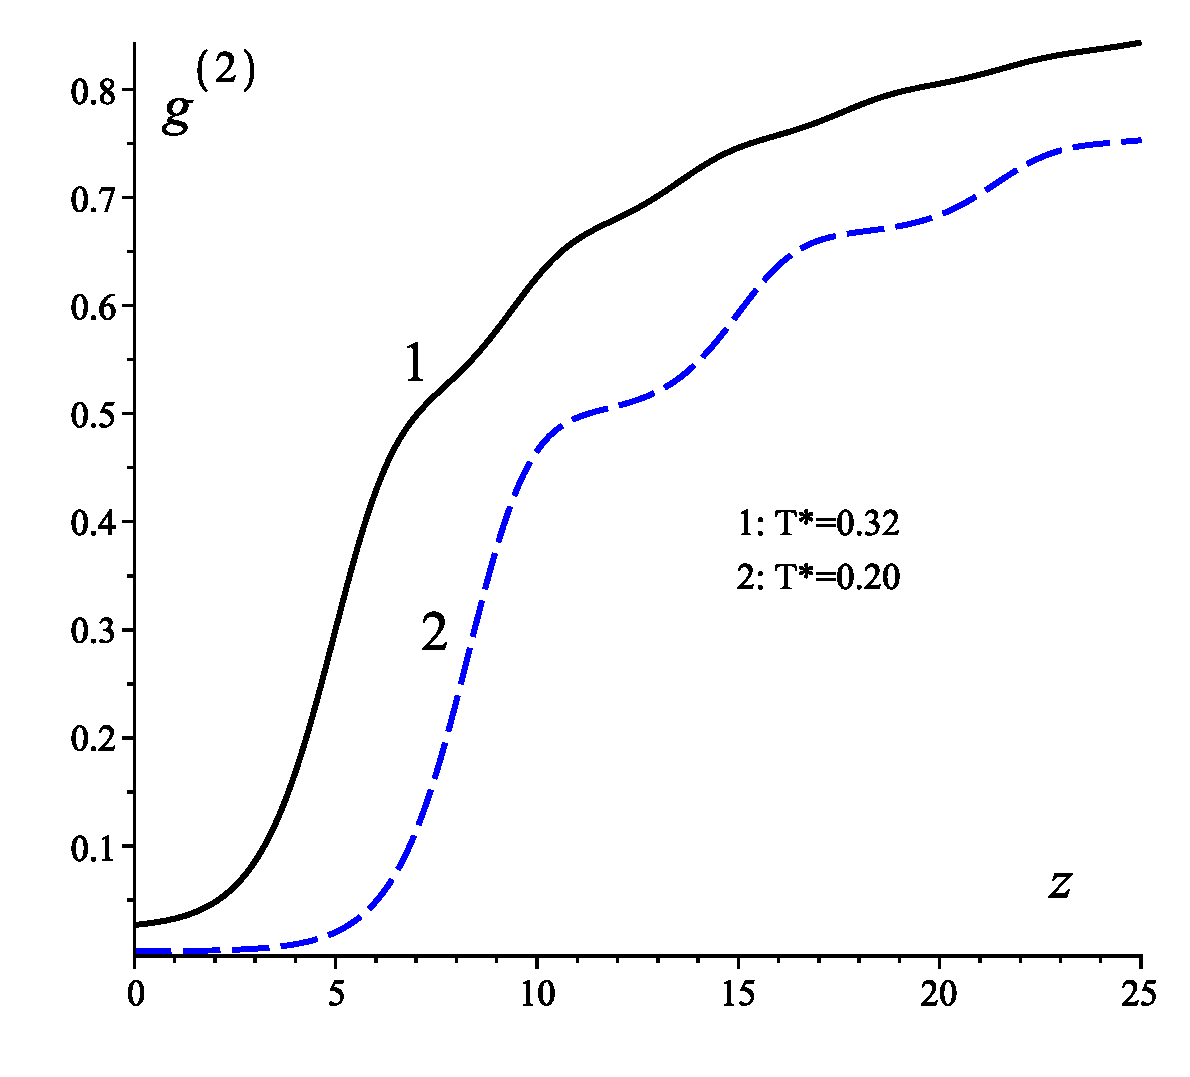
\includegraphics[width=0.7\textwidth,angle=0]{g2_vs_z}
	\caption{Pair distribution function $g^{(2)}$ versus $\bar{z}$.}
	\label{fig:g2_z}
\end{figure}
\begin{figure}[htbp]
	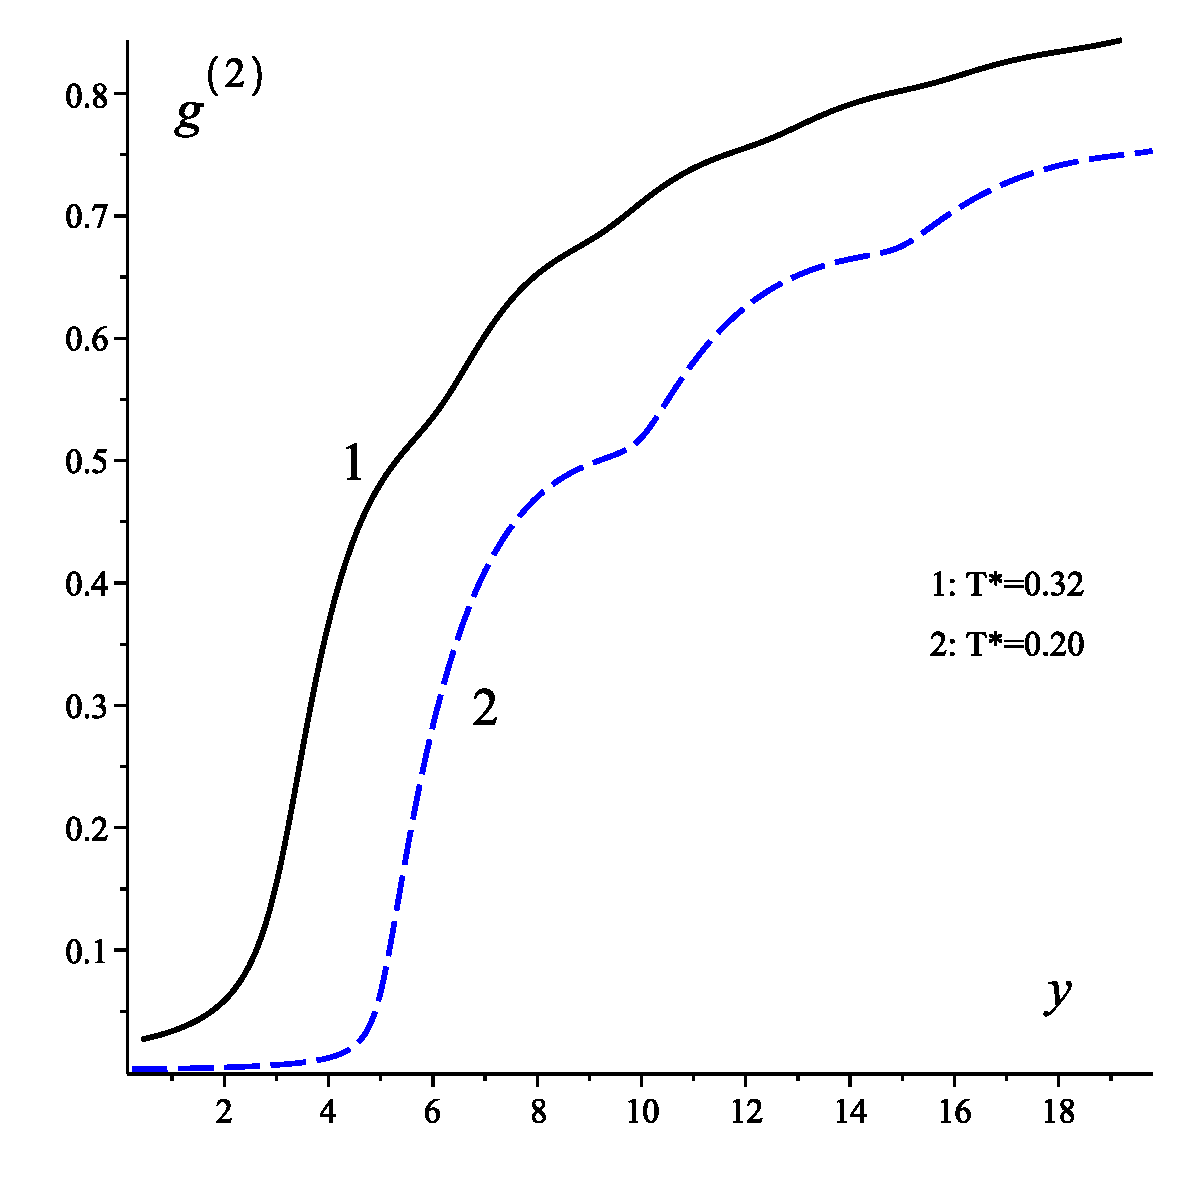
\includegraphics[width=0.7\textwidth,angle=0]{g2_vs_y}
	\caption{Pair distribution function $g^{(2)}$ versus $\bar{y}$.}
	\label{fig:g2_y}
\end{figure}

\begin{figure}[htbp]
	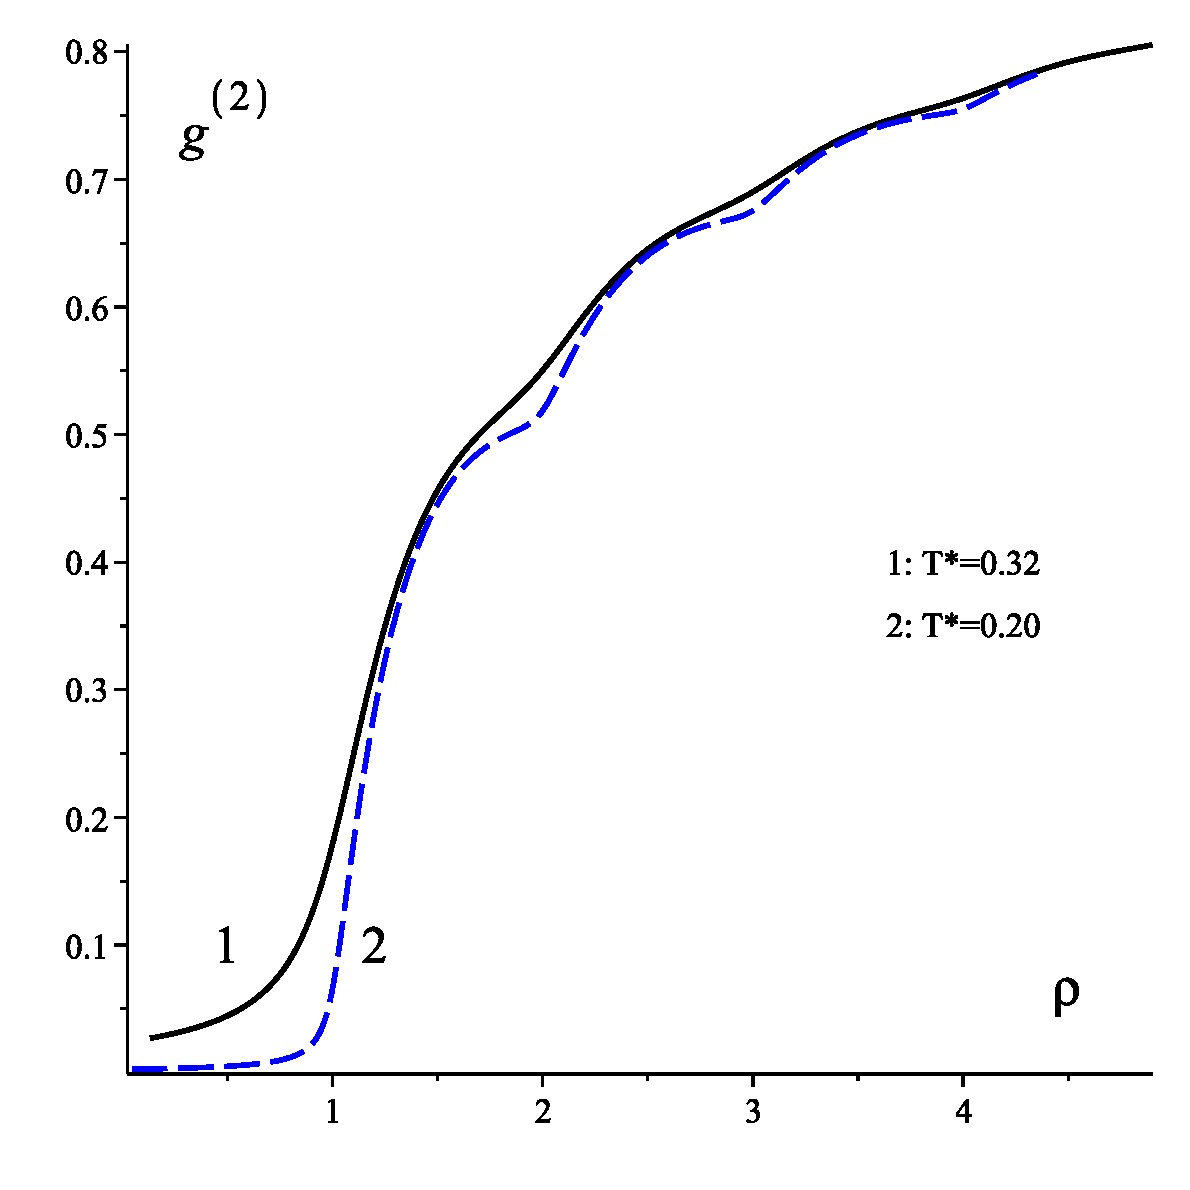
\includegraphics[width=0.7\textwidth,angle=0]{g2_vs_rho}
	\caption{Pair distribution function $g^{(2)}$ versus $\rho$.}
	\label{fig:g2_rho}
\end{figure}

\begin{figure}[htbp]
	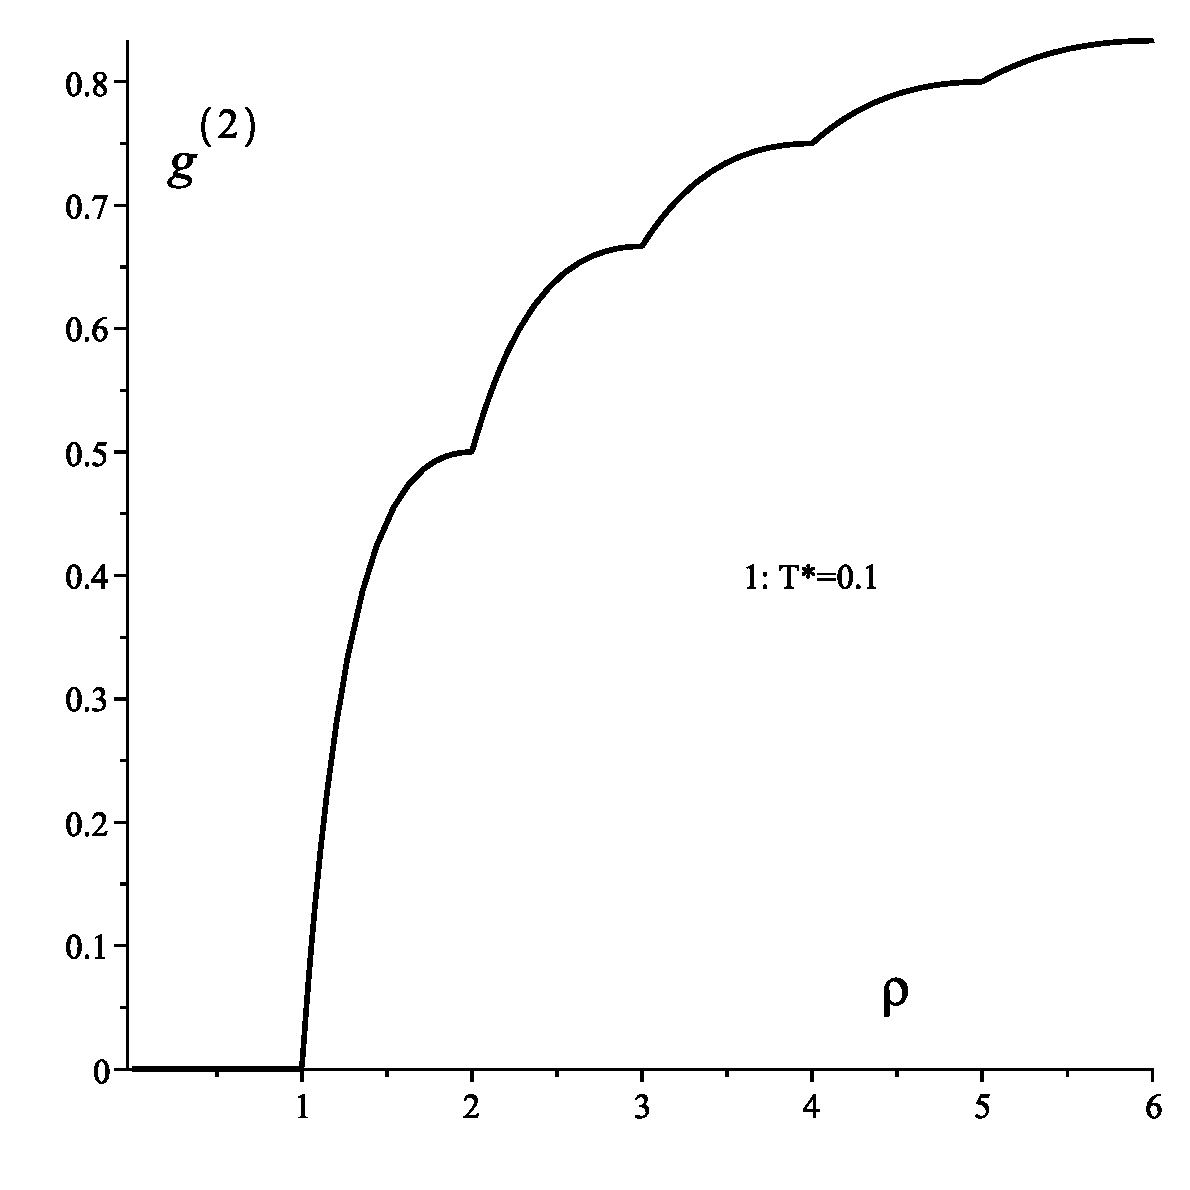
\includegraphics[width=0.7\textwidth,angle=0]{g2_vs_rho_low_temp}
	\caption{Pair distribution function $g^{(2)}$ versus $\rho$ at low temperature $T^*=0.1$.}
	\label{fig:g2_rho_low_temp}
\end{figure}

In Figure~\ref{fig:g2_z} the pair distribution function is shown as a function of $\bar{z}$ for two different values of temperature: $T^*=0.32$, which is above the range of critical temperatures, and $T^*=0.20$, which is below the range of critical temperatures. 

In Figure~\ref{fig:g2_y} the pair distribution function is shown as a function of $\bar{y}$ for the same temperatures.

In Figure~\ref{fig:g2_rho} the pair distribution function is shown as a function of density $\rho$ for the same temperatures.

Very interesting behavior of $g^{(2)}$ is observed in Figure~\ref{fig:g2_rho_low_temp}, where the dependency on density is presented in the low temperature limit, namely for $T^*=0.1$ 

The dependence of the pair distribution function on the chemical potential $\beta\mu$ is shown in Firugre~\ref{fig:g2_mu}.
\begin{figure}[htbp]
	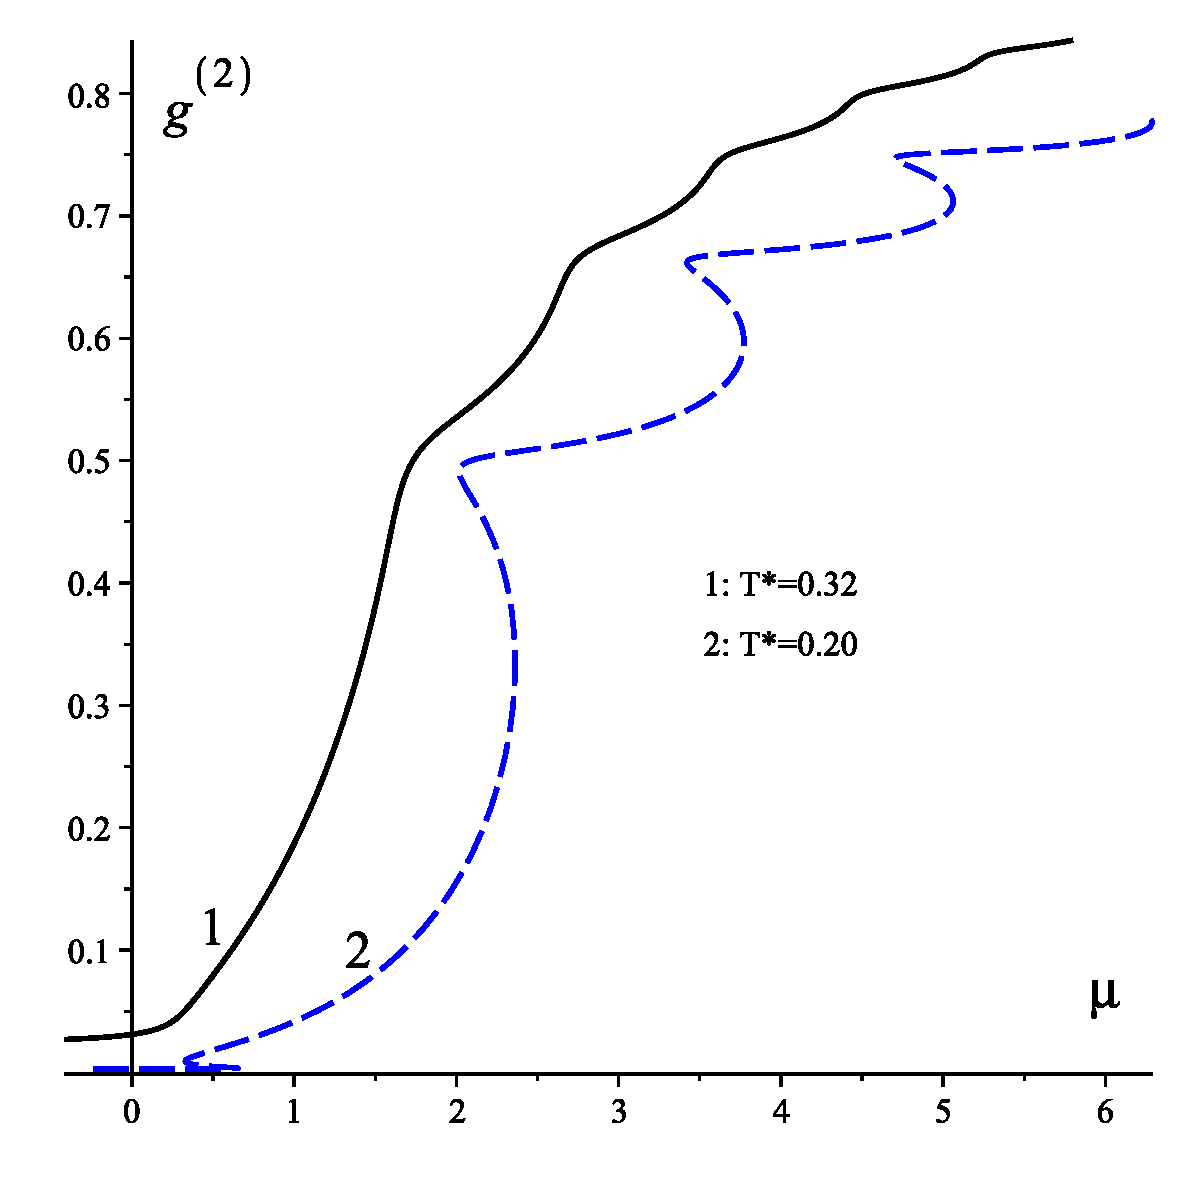
\includegraphics[width=0.7\textwidth,angle=0]{g2_vs_mu}
	\caption{Pair distribution function $g^{(2)}$ versus $\beta\mu$.}
	\label{fig:g2_mu}
\end{figure}

\begin{figure}[htbp]
	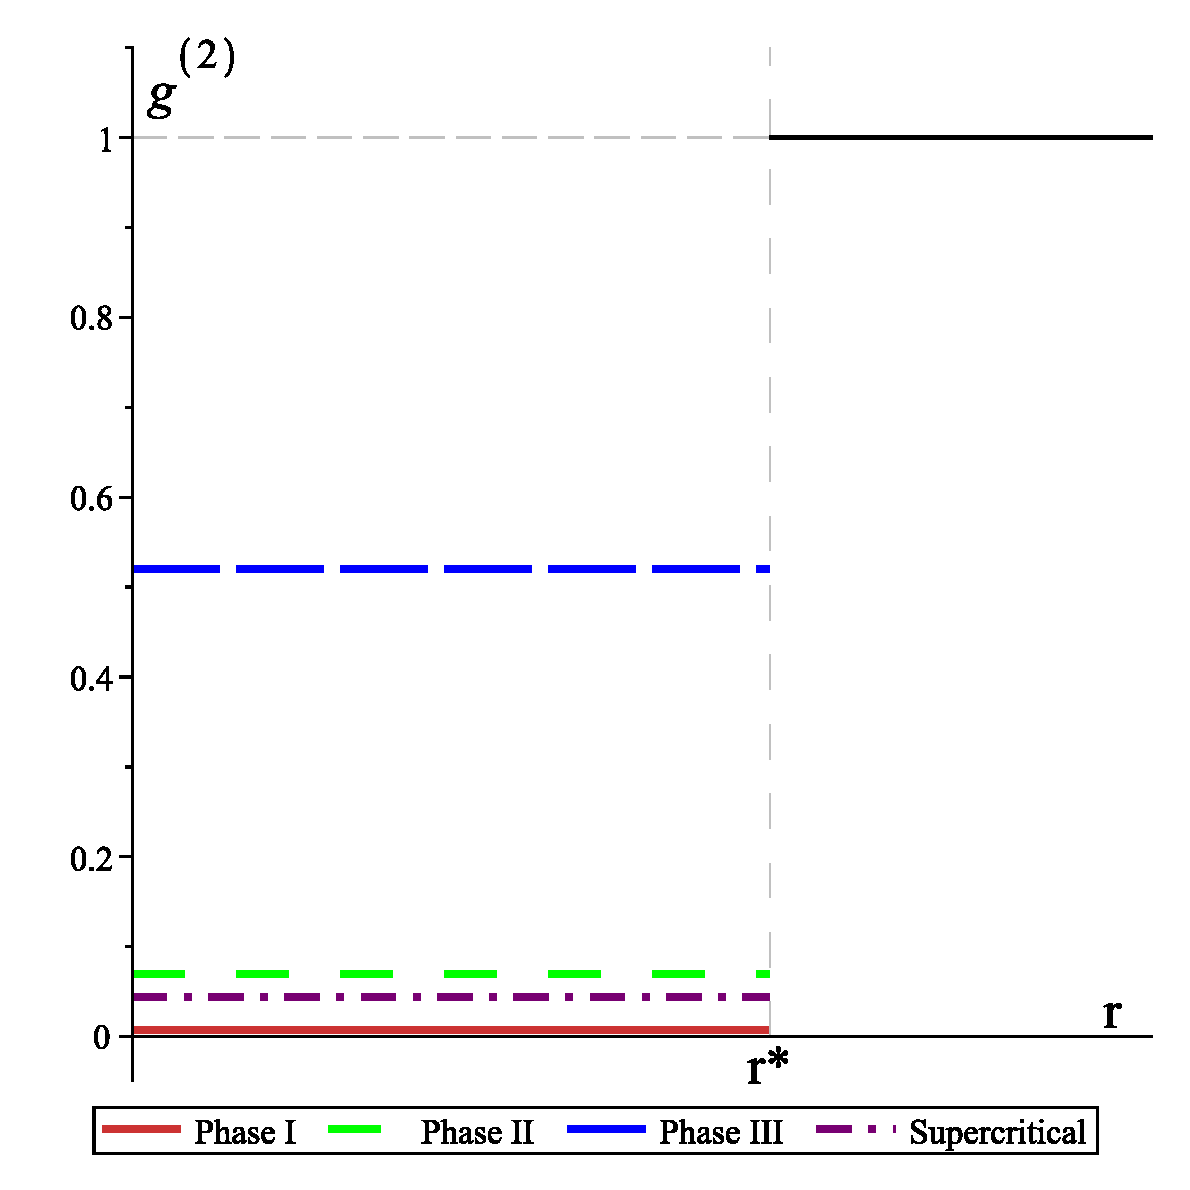
\includegraphics[width=0.6\textwidth,angle=0]{g2_vs_r}
	\caption{Pair distribution function $g^{(2)}$ as a function of separation $r$. The quantity $r^*$ denotes distance from the point with coordinate $x_1$ to the boundary of the cubic cell in the direction of $x_2$. Phase I - $T = 0.925T_c,$ $\rho^*=0.1$; Phase II - $T = 0.8T_c,$ $\rho^* = 1.0$; Phase III - $T = 0.8T_c,$ $\rho^* = 2.0$; Supercritical - $T = 1.257T_c,$ $\rho^* = 0.5$.}
	\label{fig:g2_r}
\end{figure}

\begin{figure}[htbp]
	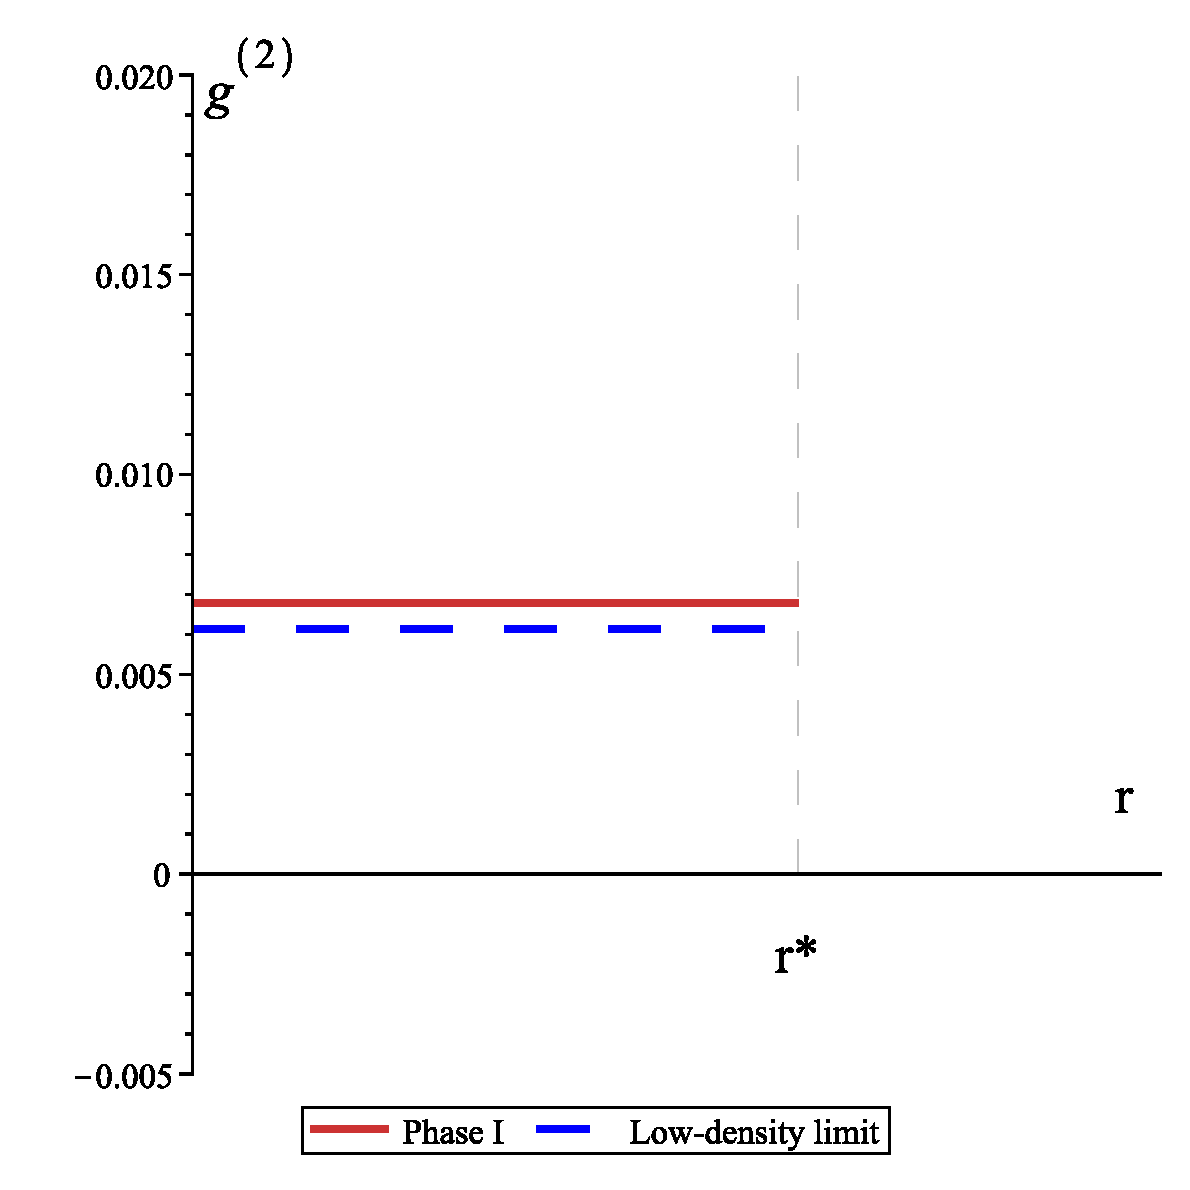
\includegraphics[width=0.6\textwidth,angle=0]{g2_vs_r_low_dens}
	\caption{Pair distribution function $g^{(2)}$ as a function of separation $r$. The quantity $r^*$ denotes distance from the point with coordinate $x_1$ to the boundary of the cubic cell in the direction of $x_2$. Phase I - $T = 0.925T_c,$ $\rho^*=0.1$; Low-density limit - $\exp(-pa)$ with $p=4.2464$ that corresponds to $T = 0.925T_c$.}
	\label{fig:g2_r_low_dens}
\end{figure}

The spatial dependency of $g^{(2)}(x_1, x_2)$ for the cell model with Curie-Weiss interaction can be presented as a step function. While $x_1$ and $x_2$ are located within one cell, $g^{(2)}$ takes on a value that is dependent of the temperature and chemical potential (or of density). However as soon as the coordinates of two particles belong to different cells, $g^{(2)}$ becomes unity.
In Figure~\ref{fig:g2_r} such step dependency is illustrated for different values of temperature and density. The temperature and density are selected to correspond to Phase I, Phase II, Phase III, and to a supercritical region over ``Phase I - Phase II'' the critical point. Since the value for Phase I is hardly visible in the scale of the graphic, Figure~\ref{fig:g2_r_low_dens} shows $g^{(2)}$ in Phase I in a better scale, along with the low-density limit~\eqref{eq:g2_low_limit}.

Finally, in Figure~\ref{fig:g2_E_mu} the dependence of $g^{(2)}$ on the chemical potential is compared with that of the quantity $E_0$ (which, in fact, is the pressure), for temperature below the critical one.
\begin{figure}[htbp]
	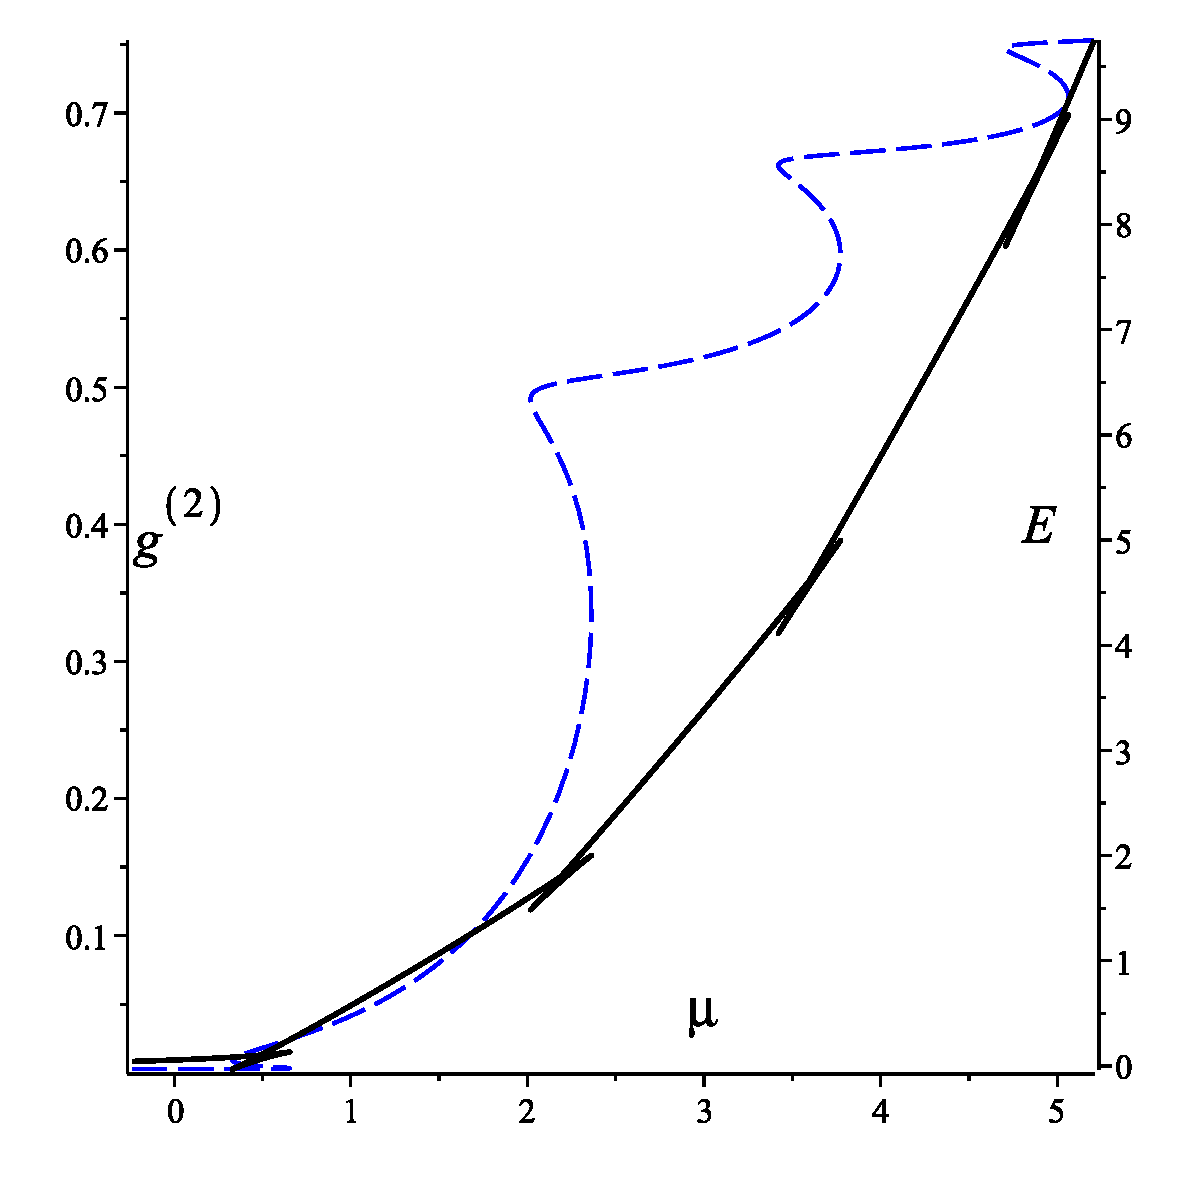
\includegraphics[width=0.6\textwidth,angle=0]{g2_vs_E_vs_mu}
	\caption{Pair distribution function $g^{(2)}$ along with quantity $E_0$ versus chemical potential $\beta\mu$. The temperature is $T^*=0.20$ (which is below the critical value).}
	\label{fig:g2_E_mu}
\end{figure}


	
	%\input{./problem_statement}
	
	\section{Conclusion}
	
	\appendix
	
	\renewcommand{\theequation}{A.\arabic{equation}}
	\setcounter{equation}{0}
	
	%\bibliographystyle{plain}
	%\bibliographystyle{longbibliography}
	% \bibliographystyle{nature}
	\bibliographystyle{cmpj}
	\bibliography{fluids_cv,books_romanik_bibliography}
	
\end{document}